\documentclass[12pt]{article}
\usepackage{ucs}
\usepackage[utf8x]{inputenc}
\usepackage[turkish,english]{babel}
\usepackage{graphicx}
\usepackage{url}
\usepackage[sc]{mathpazo}
\linespread{1.05}
\usepackage[T1]{fontenc}
\usepackage[a2paper,margin=1cm]{geometry}
\usepackage{shapepar}
\pagestyle{empty}

\author{Mehmet Atakan Gürkan}
\title{}
\date{}
\newcommand\almleftshape{
   {0}
   {0}b{0}
\\ {0}t{0}{7}
\\ {17}t{0}{11.5}
\\ {19}t{0}{11.7}
\\ {21}t{0}{11.7}
\\ {24}t{0}{11.3}
\\ {34}t{0}{8.3}
\\ {41}t{0}{4.4}
\\ {42}e{0}}
\newcommand\almrightshape{
   {12}
   {0}b{0}
\\ {0}t{3.2}{6.8}
\\ {1}t{4}{6}
\\ {5}t{2.6}{7.4}
\\ {10}t{1.0}{9}
\\ {15}t{-0.6}{10.6}
\\ {17}t{-1}{11.0}
\\ {19}t{-1.2}{11.2}
\\ {21}t{-1}{11.0}
\\ {27}t{0}{10.0}
\\ {41}t{3.5}{6.5}
\\ {42}e{10}}
\begin{document}
%\maketitle
\shorthandoff{=}
\centerline{\raisebox{-1in}{\includegraphics[clip,height=2.3975in]{afl_4_1}}
     \fontsize{40pt}{40pt}\selectfont
     \quad Ankara Fen Lisesi için Gökyüzü Almanağı \quad
\raisebox{-1in}{\includegraphics[clip,height=2.3975in]{afl_4_1}}}
\vskip -1cm
\noindent
\centerline{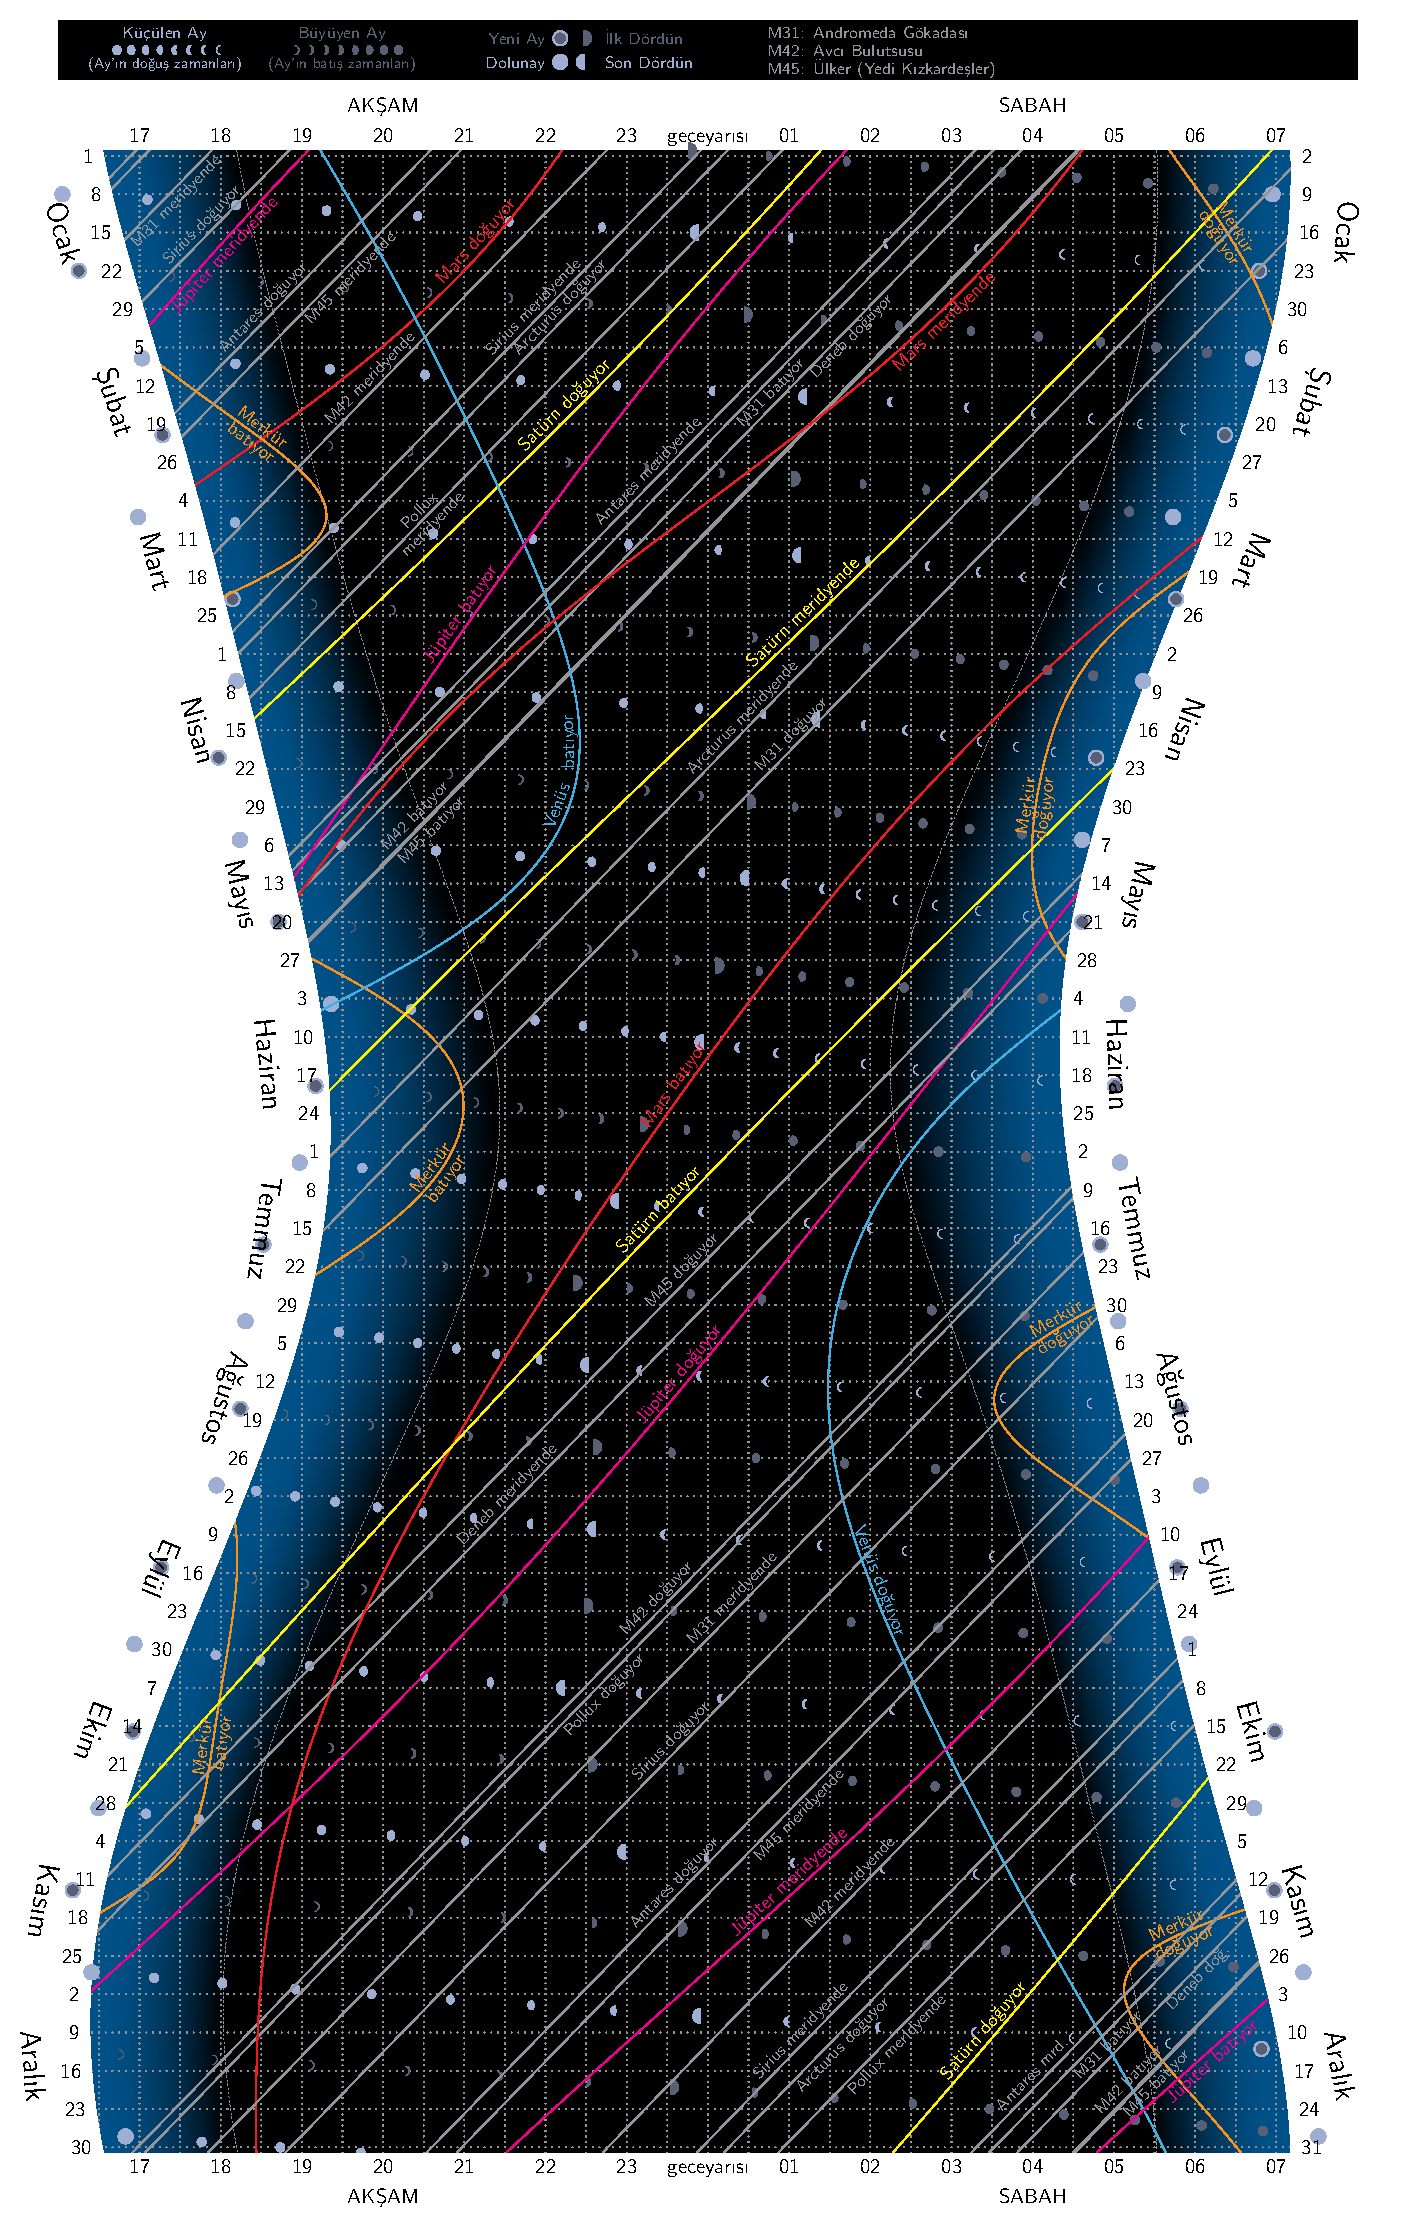
\includegraphics[clip,height=0.9\textheight]{almanac_2012_AFL}}

%\centerline{\raisebox{1in}{\includegraphics[clip,height=1.3975in]{afl_4_1}}
%     \fontsize{40pt}{40pt}\selectfont
%     \quad Ankara Fen Lisesi için Gökyüzü Almanağı \quad
%\raisebox{1in}{\includegraphics[clip,height=1.3975in]{afl_4_1}}}
%\vskip -2cm
%\noindent
%\centerline{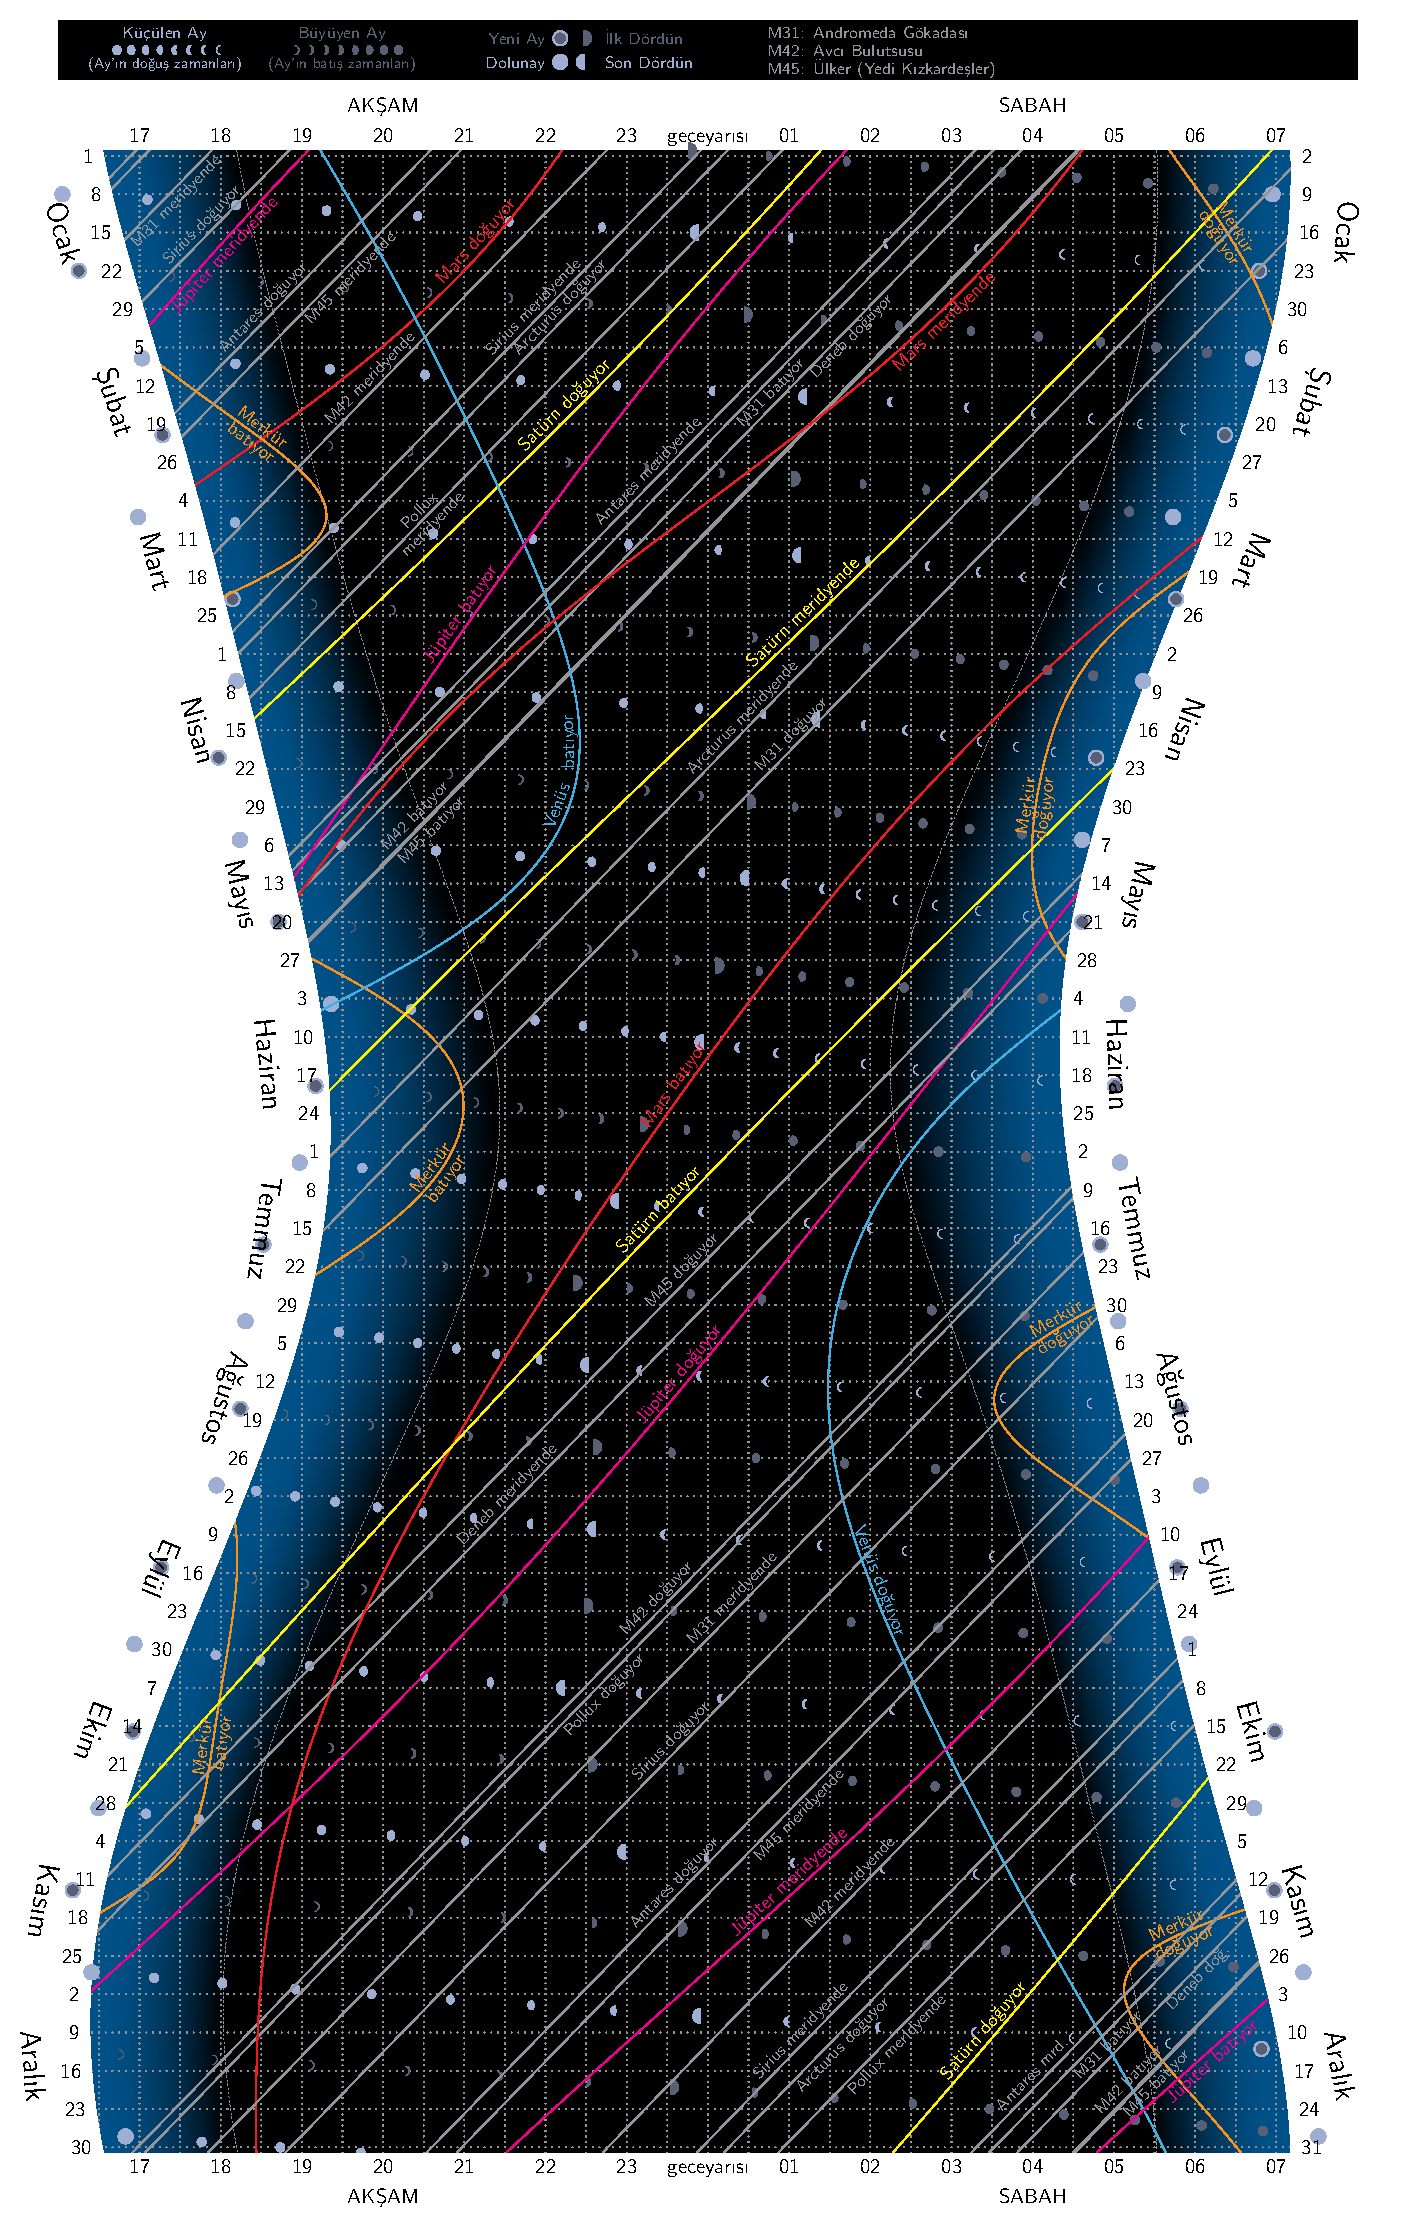
\includegraphics[clip,height=0.9\textheight]{almanac_2012_AFL}}

\vskip -0.9\textheight \vskip10.5cm
\noindent
\cutout{l}(0cm,0pt)
\shapepar{\almleftshape}{\fontsize{13pt}{13pt}\selectfont
\selectlanguage{turkish}
\hskip0.4cm\textbf{Çizelgenin Kullanımı}\\
Bu çizelge 2012 yılı için, Ankara Fen Lisesi'nde çeşitli
gök cisimlerinin doğma, meridyenden (gökyüzünde ulaştıkları en
yüksek noktadan) geçme ve batma zamanlarını, alacakaranlığın
sonuyla başlangıcını ve Ay'ın evrelerini veriyor.  Dikey eksen
günleri, yatay eksen gece boyunca zamanı gösteriyor.  Gece içinde
yarımşar saatlik aralıklar ve yıl içinde Pazar akşamlarını
Pazartesi sabahlarına bağlayan geceler noktalı çizgilerle
belirtiliyor. Düşey olarak iki nokta arası bir güne, yatay olarak
iki nokta arası beş dakikaya karşılık geliyor.\\
Bir örnek olarak 9 Mart gecesinin olaylarına bakarsak: İlk olarak,
sol tarafta 11 Mart'a karşılık gelen noktanın üstünde yaklaşık
olarak 9 Mart'a karşılık gelen noktayı bulmak gerekiyor. Buradan
sağa doğru ilerlediğimizde 18:30 civarında Avcı Bulutsusu'nun
meridyenden geçeceğini görüyoruz. Bunun ardından 19:30'da
Merkür batıyor, 19:45 civarında Sirius meridyenden geçiyor ve
20:00 civarında Arcturus doğuyor. Bu bilgilerden Güneş battığı
zaman Orion Bulutsusu, Merkür ve Sirius'un ufkun üzerinde olduğunu
da anlıyoruz. Sağa doğru ilerledikçe, belli saatlerde pekçok
gökcisminin doğduğunu, meridyenden geçtiğini ve battığını
görüyoruz. 19:40 civarında gördüğümüz Ay sembolü, Ay'ın
doğuş zamanını gösteriyor ve bir sonraki gece Ay'ın daha
küçük olacağını belirtiyor. Son olarak 19:35 ve 4:50 civarında
gördüğümüz kesikli çizgiler sırasıyla alacakaranlığın
bitmesi ve başlamasını belirtiyor. Bu noktalar Güneş'in ufkun
18$^\circ$ altında kaldığı anlara karşılık geliyor.\\
Çizelgede verilen doğma ve batma zamanları, ufuk çizgisinin önünde bir engel
olmadığını varsayıyor. Eğer böyle bir engel varsa, her bir
açı derecesi yükseklik için doğma zamanı 4 dakika geç, batma zamanı da
aynı miktarda erken olacak. Benzer biçimde, yüksek bir noktadan gözlem
yapıldığı için ufuk çizgisi olması gerekenin altında ise, doğma ve batma
zamanlarının düzeltilmesi gerekecek.\\
Not: Yaz saati uygulamasının olduğu zamanlarda,
çizelgedeki zamanlara
bir saat eklemek gerekiyor.\\
~}
\vskip -6.7cm
\cutout{r}(2em,6cm)
\shapepar{\almrightshape}{\fontsize{13pt}{13pt}\selectfont
\selectlanguage{english}
\hskip 1.2cm\textbf{Bazı Gök Olayları}\\
6 Haziran 2012 Venüs Geçişi:\\
Bundan önce 8 Haziran 2004 tarihinde izlediğimiz Venüs geçişi bu sefer 6
Haziran 2012'de gerçekleşecek. Bundan sonraki ilk Venüs geçişi içinse
yaklaşık
\hskip 1.2cm\textbf{Göktaşı Yağmurları}\\
3-4 Ocak: Quadrantid (Dörtlük)\\
22-23 Nisan: Lyrid (Lir) 
\\ ~}
\vskip 46.9cm \footnotesize

{\hfill M. Atakan Gürkan ('92) \quad \url{https://github.com/atakan/PySkyAlmanac/AFL}}
\end{document}
